% 第 18 题三棱锥 V-ABC：按固定源内容流矢量层精确值复刻（1 pt → 0.03515 cm，与全库同制）。
% 原点取 AB 中点 O（源页 (332.8438, 642.4805) pt），y 向上。
% 源实测：AB 水平长 113.3437（56.6719 pt/单位＝题设 2 单位）；△VAB 足尺等边（VA/VB 互差 ≤0.002、VO=98.1563＝√3/2·AB）；
% OC 为标准斜二测（左下 45°、深度折半 28.3312＝0.5 单位）；M 为 VA 中点（差 ≤0.0001）。
% 实线 6 条（VA、VB、VC、AC、BC、CM）；虚线 3 条（AB 被遮底棱、OM、OC）节距 2.98883/2.98883；无箭头、无填充。
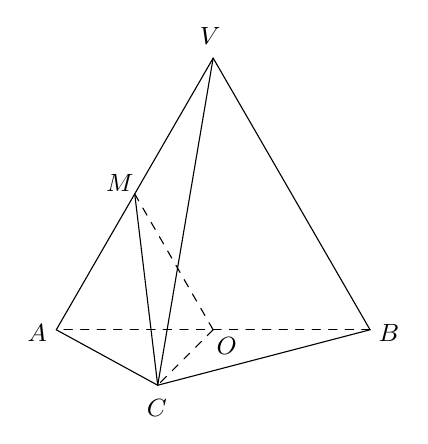
\begin{tikzpicture}[x=0.03515cm,y=0.03515cm,every node/.style={font=\small,inner sep=0pt},
  gl/.style={line width=0.3985bp,line cap=round,line join=round}]
% ===== 实线 6 条 =====
\draw[gl] (-56.6719,0)--(-20.0313,-20.0351);   % A→C
\draw[gl] (56.6718,0)--(-20.0313,-20.0351);    % B→C
\draw[gl] (0,98.1563)--(-56.6719,0);           % V→A
\draw[gl] (0,98.1563)--(56.6718,0);            % V→B
\draw[gl] (0,98.1563)--(-20.0313,-20.0351);    % V→C
\draw[gl] (-20.0313,-20.0351)--(-28.3360,49.0781); % C→M
% ===== 虚线 3 条（被遮棱与内部辅助线）=====
\draw[gl,dash pattern=on 2.98883pt off 2.98883pt] (56.6718,0)--(-56.6719,0);          % B→A
\draw[gl,dash pattern=on 2.98883pt off 2.98883pt] (0,0)--(-28.3360,49.0781);           % O→M
\draw[gl,dash pattern=on 2.98883pt off 2.98883pt] (0,0)--(-20.0313,-20.0351);          % O→C
% ===== 六顶点标签（照源字形包围盒中心定位）=====
\node at (-1.0388,106.0605) {\(V\)};
\node at (-33.7238,52.9255) {\(M\)};
\node at (-63.5388,-1.1045) {\(A\)};
\node at (63.5312,-1.1045) {\(B\)};
\node at (4.9112,-6.0345) {\(O\)};
\node at (-20.2888,-28.1195) {\(C\)};
\end{tikzpicture}
